\question[14] 设函数$f(x)=sinx$,$x \in R$.
\begin{subquestions}
    \subquestion $($\Romannum{1}$)$已知$ \theta  \in [0 , 2 \pi )$,函数$f(x+ \theta )$是偶函数,求$ \theta $的值;
    \subquestion $($\Romannum{2}$)$求函数$y=[f(x+ \dfrac { \pi }{12} )] ^{2} +[f(x+ \dfrac { \pi }{4} )] ^{2}$的值域.
\end{subquestions}
\begin{solution}{6cm}

\end{solution}



\question[15] 如图,已知三棱柱$ABC-A _{1} B _{1} C _{1}$,平面$A _{1} ACC _{1}  \perp $平面$ABC$,$ \angle ABC=90^{\small \circ}$,$ \angle BAC=30^{\small \circ}$,$A _{1} A=A _{1} C=AC$,$E$,$F$分别是$AC$,$A _{1} B _{1}$的中点.
\begin{subquestions}
    \subquestion $($\Romannum{1}$)$证明:$EF \perp BC$;
    \subquestion $($\Romannum{2}$)$求直线$EF$与平面$A _{1} BC$所成角的余弦值.
\end{subquestions}
\begin{center}
    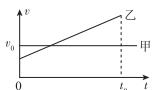
\includegraphics[]{img/image1.jpeg}
\end{center}
\begin{solution}{6cm}

\end{solution}



\question[15] 设等差数列$\{a _{n} \}$的前$n$项和为$S _{n}$,$a _{3} =4$,$a _{4} =S _{3} .$数列$\{b _{n} \}$满足:对每个$n \in N ^{*}$,$S _{n} +b _{n}$,$S _{n+1} +b _{n}$,$S _{n+2} +b _{n}$成等比数列.
\begin{subquestions}
    \subquestion $($\Romannum{1}$)$求数列$\{a _{n} \}$,$\{b _{n} \}$的通项公式;
    \subquestion $($\Romannum{2}$)$记$c _{n} = \sqrt { \dfrac {a_{n}}{2b_{n}}}$,$n \in N ^{*}$,证明:$c _{1} +c _{2} + \cdots +c _{n}  \lt  2 \sqrt {n}$,$n \in N ^{*}$.
\end{subquestions}
\begin{solution}{6cm}

\end{solution}



\question[12] 如图,已知点$F(1 , 0)$为抛物线$y ^{2} =2px(p  \gt  0)$的焦点$.$过点$F$的直线交抛物线于$A$,$B$两点,点$C$在抛物线上,使得$\triangle ABC$的重心$G$在$x$轴上,直线$AC$交$x$轴于点$Q$,且$Q$在点$F$的右侧$.$记$\triangle AFG$,$\triangle CQG$的面积分别为$S _{1}$,$S _{2}$.
\begin{subquestions}
    \subquestion 求$p$的值及抛物线的准线方程;
    \subquestion 求$ \dfrac {S_{1}}{S_{2}}$的最小值及此时点$G$点坐标.
\end{subquestions}

\begin{solution}{6cm}

\end{solution}
\question[15] 已知实数$a\neq 0$,设函数$f(x)=a\ln x+ \sqrt {1+x}$,$x  \gt  0$.
\begin{subquestions}
    \subquestion $($\Romannum{1}$)$当$a=- \dfrac {3}{4}$时,求函数$f(x)$的单调区间;
    \subquestion $($\Romannum{2}$)$对任意$x \in \Big[ \dfrac {1}{\mathrm e^{2}} , + \infty \Big)$均有$f(x)\leqslant \dfrac { \sqrt {x}}{2a}$,求$a$的取值范围.
    \subquestion 注意:$\mathrm e=2.71828 \cdots  \cdots $为自然对数的底数.
\end{subquestions}
\begin{solution}{6cm}

\end{solution}
